\subsection{Turing Test}
124 subjects, 3 B\&W + 4 colored.

i risultati sono diversi perchè le foto B\%W sono scattate con una diversa tecnologia rispetto alle foto a colori

Figure \ref{fig:turing}
\begin{figure}[h]
	\centering
	\captionsetup[subfigure]{labelformat=empty}
	\begin{subfigure}[b]{0.1\textwidth}
		\begin{adjustwidth}{-1.1cm}{}
		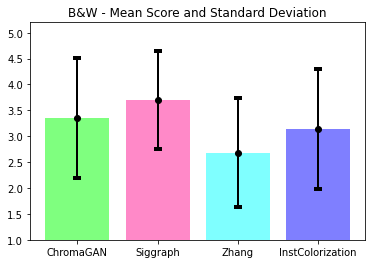
\includegraphics[width=4cm]{bw turing.png}
		\end{adjustwidth}
	\caption{B\&W}
	\end{subfigure}
\hspace{2.3cm}
	\begin{subfigure}[b]{0.1\textwidth}
		\begin{adjustwidth}{-1.1cm}{}
			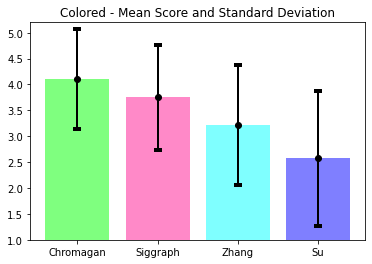
\includegraphics[width=4cm]{col turing.png}
		\end{adjustwidth}
		\caption{Colored}
	\end{subfigure}
	\caption{{\small Mean scores obtained with the colorization on black and white photographs and originally colored images.}}
	\label{fig:turing}
\end{figure}